% Refusals for malware and for pathogens live in the same layer, so injection defeats both.
% ---------------------------------------------------------------------------
% style.tex --- shared preamble for every figure in book/figures/tikz/
%
% One style for all figures: Latin Modern, thin black lines, a light grey
% fill, and one accent colour used only to mark what is untrusted or wrong.
% Build with scripts/build_figures.sh; see book/figures/README.md.
% ---------------------------------------------------------------------------
\documentclass[tikz,border=6pt]{standalone}
\usepackage[T1]{fontenc}
\usepackage{lmodern}
\usetikzlibrary{arrows.meta,positioning,shapes.geometric,calc,fit,backgrounds}

\hyphenpenalty=10000   % short lines in boxes: ragged, never hyphenated

\definecolor{lightgrey}{gray}{0.92}
\definecolor{accent}{HTML}{9B2D20}

\tikzset{
  every picture/.style={
    line width=0.6pt,
    font=\small,
    >={Stealth[length=5pt,width=4pt]},
    node distance=14pt and 24pt,
  },
  % shapes
  box/.style={draw, rectangle, inner xsep=8pt, inner ysep=5pt,
              minimum height=22pt, align=center},
  grey/.style={box, fill=lightgrey},
  rounded/.style={box, rounded corners=9pt},
  decision/.style={draw, diamond, aspect=2.4, inner sep=1.5pt, align=center},
  group/.style={draw, dashed, rounded corners=5pt, inner sep=7pt},
  % text
  tag/.style={font=\footnotesize, align=center, inner sep=2pt},
  note/.style={font=\footnotesize\itshape, align=center, inner sep=2pt},
  code/.style={font=\small\ttfamily},
  codetag/.style={font=\footnotesize\ttfamily, align=center, inner sep=2pt},
  title/.style={font=\small\scshape, align=center, inner sep=2pt},
  % lines
  arrow/.style={->},
  back/.style={->, dashed},
  thin/.style={line width=0.4pt, gray},
  % the one accent, for what is untrusted, wrong or missing
  bad/.style={accent},
  badbox/.style={box, draw=accent, text=accent},
}

\begin{document}
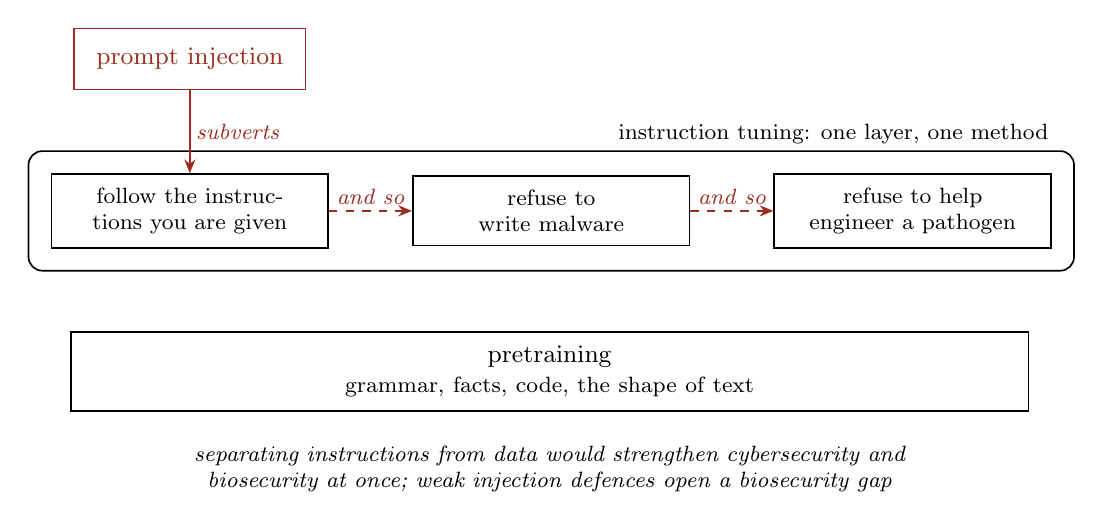
\begin{tikzpicture}[node distance=10pt and 30pt, item/.style={box, text width=84pt, align=center, font=\footnotesize}]
  \node[box, text width=330pt, align=center] (pre) at (0,0) {pretraining\\ \footnotesize grammar, facts, code, the shape of text};
  \node[item] (rules) at (-130pt,58pt) {follow the instructions you are given};
  \node[item, right=of rules] (mal) {refuse to write malware};
  \node[item, right=of mal] (bio) {refuse to help engineer a pathogen};
  \node[group, solid, fit=(rules) (mal) (bio), inner sep=8pt, label={[tag]above right:instruction tuning: one layer, one method}] (layer) {};
  \node[badbox, above=30pt of rules] (inj) {prompt injection};
  \draw[->, bad] (inj) -- node[note, right, text=accent] {subverts} (rules);
  \draw[->, bad, dashed] (rules) -- node[note, above, text=accent] {and so} (mal);
  \draw[->, bad, dashed] (mal) -- node[note, above, text=accent] {and so} (bio);
  \node[note, below=10pt of pre, text width=330pt]
    {separating instructions from data would strengthen cybersecurity and biosecurity at once;
     weak injection defences open a biosecurity gap};
\end{tikzpicture}
\end{document}
